\chapter{Le travail réalisé}

%
%
%
\section{État de l'existant}
Quand je suis arrivé au laboratoire \textit{CIRDLES}, le cœur du logiciel avait déja été réalisé par John Zeringue, mon partenaire principal pendant ce stage. Il y avait un tableau où l'on pouvait entrer des données, et on pouvait déja génèrer un graphique avec les ellipses d'erreurs et une des lignes Concordia\footnote{On savait pas d'ailleurs à l'époque qu'il y avait plusieurs lignes Concordia. On appelait tout simplement celle qui était dans le logiciel ``La Ligne Concordia''. C'est bien plus tard que nous avons découvert qu'il y en avait plusieurs.}.

Le moment où je suis arrivé coïncide avec le moment où le Docteur Bowring nous a donné le cas d'utilisation basique du chercheur australien à implémenter. Le cas d'utilisation peut se résumer aux étapes suivantes :
\begin{enumerate}
\item Le géochronologiste a des données dans une feuille Excel qui représente des ratios et leurs inexactitudes. Il les copie.
\item Il colle les données dans \textit{Topsoil}.
\item Il demande à générer le schema, le logiciel le lui montre.
\item Il peut l'exporter au format SVG
\end{enumerate}

Après avoir passé deux jours à me renseigner sur la géochronologie en lisant une publication du Docteur Bowring et en regardant un DVD sur le sujet, %Cette phrase mérite peut-être sa propre section. Ou elle l'aura dans la quatrième partie.
J'ai commencé avec John à implémenter ce cas d'utilisation.

%
%
%
\section{L'implémentation du cas d'utilisation}
Il n'y a avait pas beaucoup de travail pour adapter le logiciel au cas d'utilisation. Pendant que John s'est occupé de l'import de données depuis \textit{Excel}, j'ai créé le \textit{ColumnSelectorView}.

%
%
\subsection{Le \textit{ColumnSelectorView}}
Dans la version d'alors du logiciel, le tableau n'avait que cinq colonnes, une pour chaque variable dont nous avions besoin pour tracer les ellipses d'erreurs. Nous avons décidé de permettre aux utilisateurs d'insérer autant de colonnes qu'ils souhaitaient depuis leur feuille de calcul Excel. Cela demandait cependant une étape supplémentaire : lier les colonnes aux variables. C'est exactement le travail du \textit{ColumnSelectorView}. 

\begin{center}
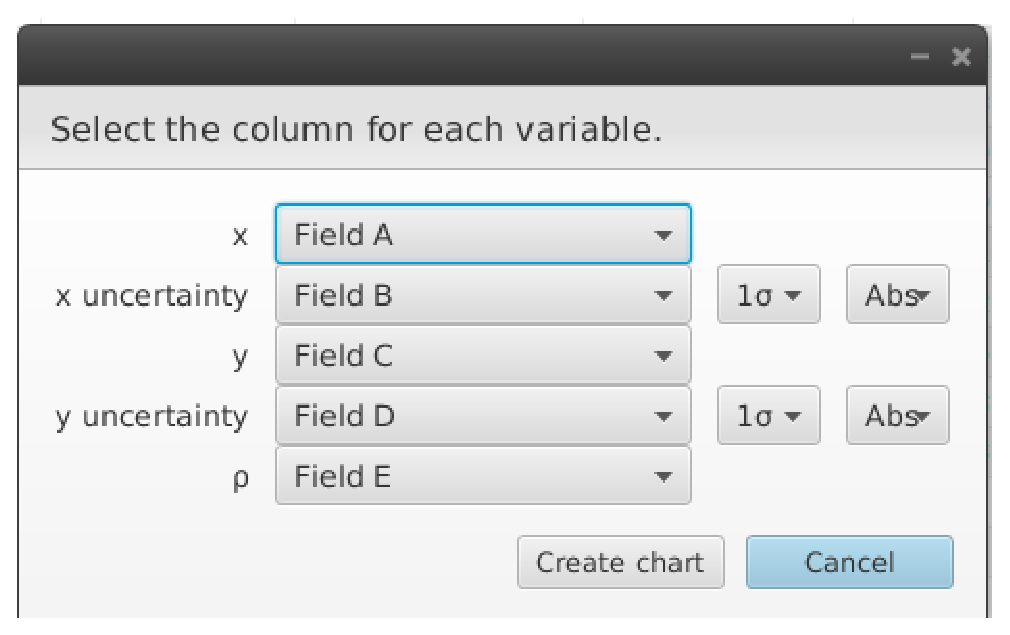
\includegraphics[width=7cm]{./illustrations/columnselectorview.eps}
\end{center}

D'un point de vue graphique cette interface n'est pas très intéressante. La façon dont je l'ai implémenté sera par contre très intéressante pour le chapitre quatre, qui portera sur \textit{ce que j'ai appris durant ce stage}. La première mouture de cette classe ne comportait pas la logique pour de la génération du schéma. Sa conceptipon était pour moi un petit utilitaire qui ne sert qu'à choisir les champs, la génération du schéma à partir du schema devait se faire autre part. Cette classe était liéà un \textit{listener}\footnote{Un listener est une interface (au sens programatique du terme) qui réagit aux signaux d'un objet en particulier. Ici, le listener génerait le schema.} qui générait le schéma, implémenté dans la classe qui gêrait le tableau. Cela faisait sens pour moi que la génération d'un graphique avec les données d'un tableau soit ordonnée par ce même tableau. Ce n'est pas faux en soit, mais il y a mieux\ldots


Quinze jours plus tard, John avait drastiquement changé la classe pour me faire comprendre que ma façon de concevoir était très démodée en supprimant l'interface \textit{ColumnSelectorInterfaceListener}.
. Laissez moi vous expliquer plus en détails.

Nous utilisons dans le projet une librairie appelée \textit{ControlsFX}. Elle ajoute des éléments d'interface graphique qui ne sont pas dans la librairie originale, ainsi que la notion d'\textbf{Actions}. Une Action est un objet qui \textit{fait quelque chose en réaction à une demande de l'utilisateur}. Un de ses avantages est qu'elle est automatiquement transformée en élément d'interface par \textit{ControlsFX}. Exemple : une boite de dialogue est liée une série d'Actions que l'utilisateur peut choisir en réaction à son affichage. C'est elle qui les tranforme automatiquement en boutons.

John a transformé ma classe qui était auparavant un simple élément affichable par \textit{JavaFX} en boite de dialogue de \textit{ControlsFX}. Elle était dorénavant mieux intégrée stylistiquement à l'interface de l'application, et surtout, elle enlevait le \textit{listener} du tableau, et donnait à la logique de génération de tableau sa propre classe : une Action. Bien plus propre.

Aujourd'hui cette Action est toujours une classe gigogne du \textit{ColumnSelectorView}, ce qui est selon toute l'équipe une place non-idéale. Il faudra bientôt que l'on déplace toutes nos actions dans un package qui leur est dédié.

%
%
\subsection{Complétion du convertisseur SVG}
Il ne restait alors plus qu'une seule tâche avant que l'implémentation du cas d'utilisation soit terminée : La conversion du graphique en un fichier SVG.

\begin{quote}
Le SVG est un format graphique vectoriel. Un fichier au format SVG contient la définition de diverses formes. Ces défintions comportent entre autre la position de la forme, la couleur de son tracé et de son remplissage, la largeur de son tracé \ldots.
\end{quote}

\begin{quote}
Un nœud (\textit{Node}) dans \textit{JavaFX} est la classe de base de n'importe quel élément affichable. La plupart du temps, on utilise des nœuds composés d'autres nœuds. Un simple bouton, par exemple, contient au moins un rectangle et un label\footnote{Nom d'un texte affiché à l'écran dans le jargon informatique}.
\end{quote}

\begin{quote}
Une scène (\textit{Scene}) est un ensemble de nœuds destinés à être affichés.
\end{quote}

J'ai repris en charge l'écriture d'un convertisseur que John avait commencé à écrire. Ce convertisseur est conçu pour pouvoir transformer n'importe quel nœud en SVG. Pour cela il parcourt tous les nœuds récursivement\footnote{La récursivité est un concept de l'informatique qui désigne la répétition d'une action entrainée par cette même action. Ici, l'action serait ``Parcourir les enfants''. Quand je \emph{parcours les enfants}, si je trouve un enfants qui en a d'autres, je \emph{parcours ses enfants}.} jusqu'à tomber sur des noeud de base qu'il convertit en éléments SVG. Nous nous en servons sur le nœud du graphique afin de le convertir en image vectoriel.

Le travail que j'ai du effectuer pour ce convertisseur est principalement un travail d'investigation. Il fallait que je trouve où et comment JavaFX définit les options graphiques des nœuds afin de les répercuter sur les élément SVG leur correspondant.

Pour cela, j'ai tout d'abord regardé comment le noeud du graphique était composé. J'ai extrait la hierarchie du nœud du graphique :

\begin{verbatim}
ConcordiaChart@b721ec6[styleClass=chart]
   Label@58eeaa1f[styleClass=label chart-title]''
      Text[text="", x=0.0, y=0.0, alignment=LEFT, origin]
   Chart$1@5109fabb[styleClass=chart-content]
      Region@3078127b[styleClass=chart-plot-background]
      XYChart$1@206ec019
          Path[elements=[], fill=null, fillRule=NON_ZERO]
          Path[elements=[MoveTo[x=100.0, y=10.0], LineTo[x=1 
          Path[elements=[MoveTo[x=297.5, y=10.0], LineTo[x=2
          Path[elements=[MoveTo[x=100.0, y=646.5], LineTo[x 
          Line[startX=0.0, startY=0.0, endX=0.0, endY=0.0, s 
          Line[startX=0.0, startY=0.0, endX=0.0, endY=0.0, s
          Group@5867eb04[styleClass=plot-content]
              Group@789d6eba
                  Path[elements=[MoveTo[x=0.0, y=-57194.0], LineTo[x Invisible
              Group@400b7196[styleClass=error-ellipse]
                  Path[elements=[MoveTo[x=1023.0, y=62.0], CubicCurv
              Group@bddd852[styleClass=error-ellipse]
                  Path[elements=[MoveTo[x=798.0, y=206.0], CubicCurv
                  Circle[centerX=775.0, centerY=221.0, radius=3.0, f
              Group@27c9ed47[styleClass=error-ellipse]
                  Path[elements=[MoveTo[x=604.0, y=481.0], CubicCurv
                  Circle[centerX=583.0, centerY=497.0, radius=3.0, f
              Group@5c612db6[styleClass=error-ellipse]
                  Path[elements=[MoveTo[x=103.0, y=598.0], CubicCurv
                  Circle[centerX=83.0, centerY=615.0, radius=3.0, fi
              Group@1e4ce279[styleClass=error-ellipse]
                  Path[elements=[MoveTo[x=810.0, y=538.0], CubicCurv
                  Circle[centerX=789.0, centerY=557.0, radius=3.0, f
              Group@5eec36db[styleClass=error-ellipse]
                  Path[elements=[MoveTo[x=433.0, y=339.0], CubicCurv
                  Circle[centerX=411.0, centerY=352.0, radius=3.0, f
      NumberAxis@2b5f1854[styleClass=axis] Horizontal 
         Label@29a340ae[styleClass=label axis-label]'xxxPb/
              Text[text="xxxPb/xxxU", x=0.0, y=0.0, alignment=LE 207pb/235u
          Path[elements=[MoveTo[x=0.0, y=0.0], LineTo[x=0.0, 
          Path[elements=[MoveTo[x=40.0, y=1.0], LineTo[x=40. 
          Text[text="0.0720000", x=0.0, y=0.0, alignment=LEF
          Text[text="0.0720500", x=0.0, y=0.0, alignment=LEF
          Text[text="0.0721000", x=0.0, y=0.0, alignment=LEF
          Text[text="0.0721500", x=0.0, y=0.0, alignment=LEF
          Text[text="0.0722000", x=0.0, y=0.0, alignment=LEF
          Text[text="0.0722500", x=0.0, y=0.0, alignment=LEF
      NumberAxis@2650091e[styleClass=axis]
          Label@2ea49c54[styleClass=label axis-label]'xxxPb/
              Text[text="xxxPb/xxxU", x=0.0, y=0.0, alignment=LE Invisible
          Path[elements=[MoveTo[x=82.0, y=636.0], LineTo[x=9
          Path[elements=[MoveTo[x=85.0, y=679.0], LineTo[x=8
          Text[text="0.0000800", x=0.0, y=0.0, alignment=LEF
          Text[text="0.0001000", x=0.0, y=0.0, alignment=LEF
          Text[text="0.0001200", x=0.0, y=0.0, alignment=LEF
          Text[text="0.0001400", x=0.0, y=0.0, alignment=LEF
          Text[text="0.0001600", x=0.0, y=0.0, alignment=LEF
          Text[text="0.0001800", x=0.0, y=0.0, alignment=LEF
          Text[text="0.0002000", x=0.0, y=0.0, alignment=LEF
          Text[text="0.0002200", x=0.0, y=0.0, alignment=LEF
      Rectangle[x=0.0, y=0.0, width=0.0, height=0.0, fil Empty
\end{verbatim}
J'ai cherché à savoir à quel élément graphique correspondait chacuns de ces éléments, en comparant leur position avec les éléments d'un fichier SVG génèré par le code existant.  Pour une meilleur compréhension de ce qui suit, une capture d'écran d'un graphique a été placé après cette liste. Le \textit{ConcordiaChart} est composé de :
\begin{itemize}
\item Un objet \textit{Label} : le titre du graphique
\item Un objet \textit{Chart}, père d'un objet \textit{XYChart} contenant :
  \begin{itemize}
  \item Des objets \textit{Path} : Les lignes horizontales et verticale formant la grille du graphique
  \item Un objet \textit{Group} : Les objets affichés sur le graphique
    \begin{itemize}
    \item La ligne de temps est l'objet \textit{Path} dans le second des \textit{Group}
    \item Les autres \textit{Group} contiennent un \textit{Path}, l'ellipse, et un \textit{Circle}, le point au milieu de l'ellipse.
    \end{itemize}
  \end{itemize}
\item Deux objets \textit{Axis}, contenant chacun :
  \begin{itemize}
  \item Un \textit{Label} : la légende de l'axe
  \item Deux éléments \textit{Path} : Les grandes et petites marques de graduation
  \item Des éléments \textit{Text} : La légende des grande graduations
  \end{itemize}
\end{itemize}

\begin{center}
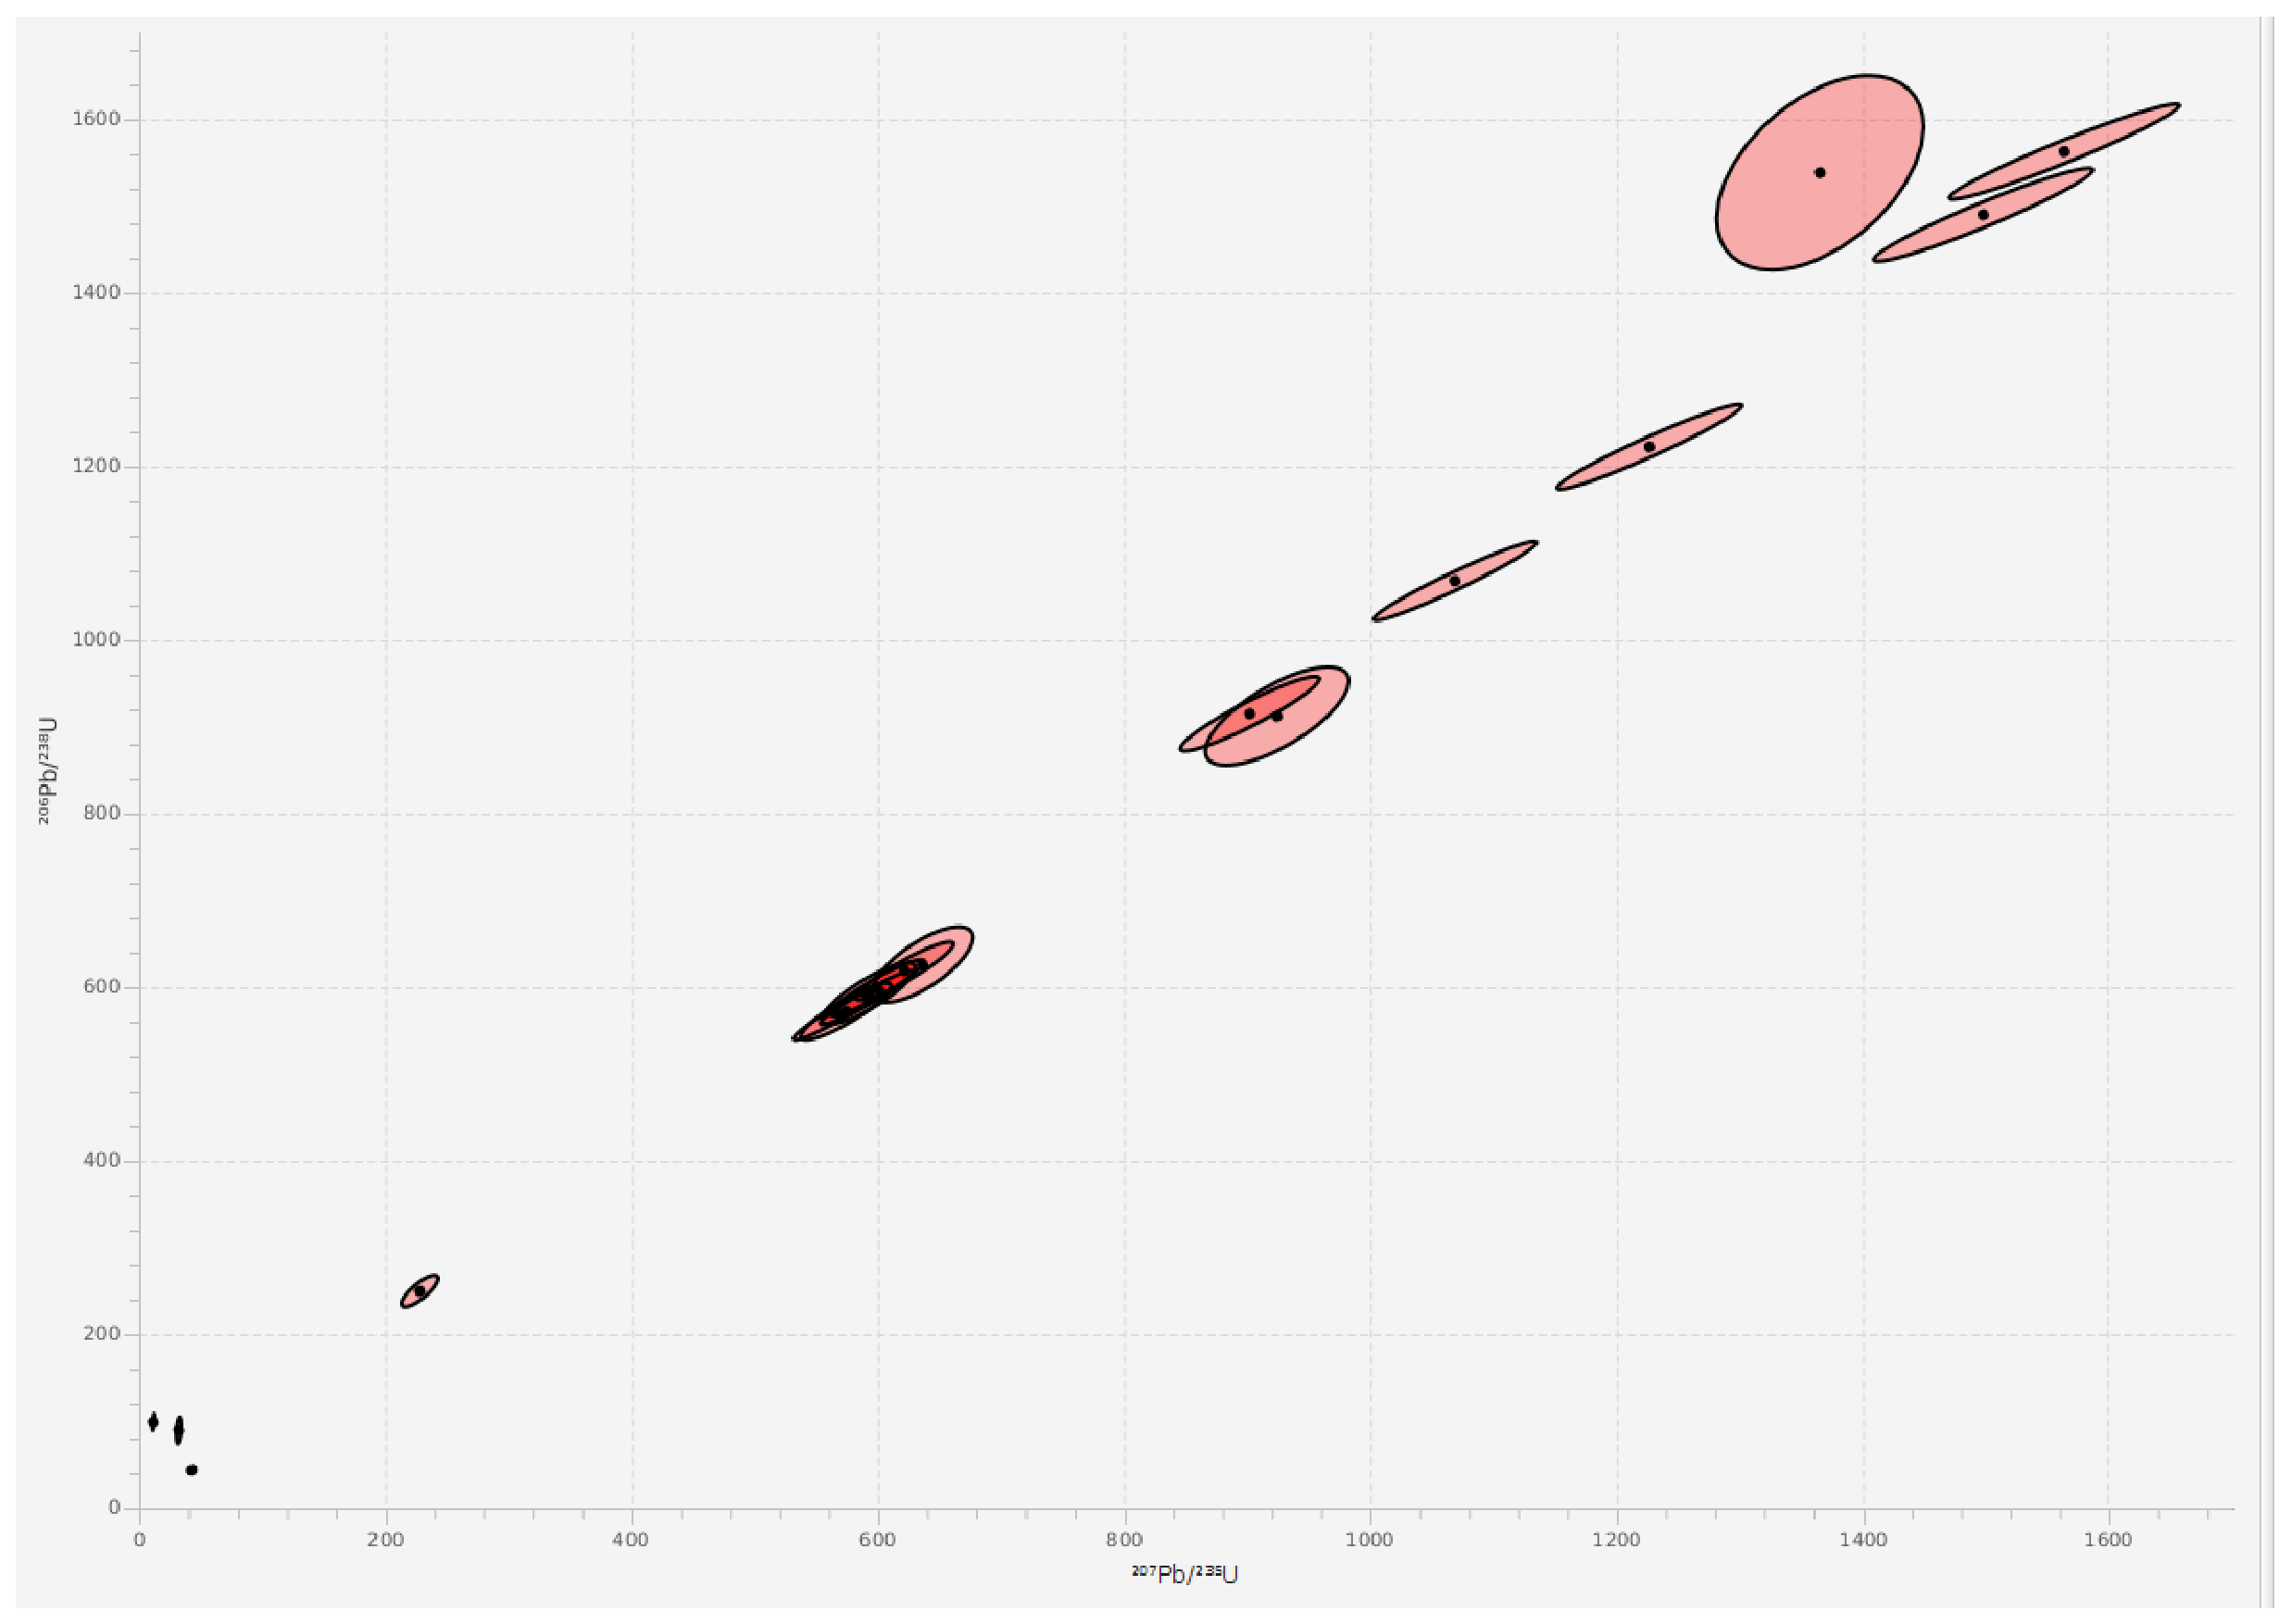
\includegraphics[width=10cm]{./illustrations/graphique.eps}
\end{center}


J'ai ensuite été chercher dans le moteur de rendu de \textit{JavaFX} la logique qui rend une scene à l'écran. Mon plan (diabolique s'il en est), était de voir où cette logique récupère les options graphiques des noeud qu'elle doit dessiner. Si mon plan a failli, me coutant quelques jours, j'ai néanmoins appris énormément sur la façon dont \textit{JavaFX} fonctionne. 

Pour résumer, le code de JavaFX est separé en deux :
\begin{enumerate}
\item La partie publique est celle que l'on utilise pour construire une scene, et plus génénalement pour intéragir avec la librairie. Elle contient aussi les \textit{Property}, dont je parlerais plus tard. Elle est sous le package %TODO noter le package avec Verbatim
\item La partie privée (joyeusement fouillie et peu commentée) a différents rôles:%TODO noter le package avec verbatim
  \begin{enumerate}	
  \item Rendre des scenes (Moteur de rendu \textit{Prism}, sur lequel je me suis particulierement penché)
  \item Unifier l'interaction avec les systèmes de fenêtrage des différents OS avec lesquels \textit{JavaFX} est compatible. (Module \textit{Glassfish})
  \item Rendre différents type de médias
  \item Rendre du HTML (Moteur basé sur \textit{Webkit})
  \item Marcher sur plusieurs threads
  \end{enumerate}
\end{enumerate}

Après la faillite de mon premier plan, j'ai procédé plus simplement. Je suis revenu aux noeuds dans la partie publique, ceux que nous manipulons quand nous créons une scène, et ait cherché les différentes options graphiques en leur sein. J'ai reussi à trouver et à orienter correctement le nom des axes et à repositionner ceux-ci, j'ai re-aligné les graduations, repositionné et affiché des lignes et des textes dans le graph.

%
%
%
\section{Réponse aux attentes de la communauté GitHub}
Le module SVG était fini. Le cas d'utilisation était implémenté. Nous étions près à montrer le fruit de notre travail aux chercheurs Australiens, ce que nous avons fait le Mercredi 21 mai par visioconférence. Ils étaient enchantés du prototype.

Le docteur Bowring a envoyé un lien vers le dépot GitHub du projet, et une petite mais active communauté s'est formée autour du projet. Ses membres nous envoient encore à ce jours des rapports de bug, des suggestions de fonctions.

Cela a bien sur beaucoup changer la dynamique de travail. Nos journées étaient à présent partagées entre réponses à la communauté, corrections rapides de bugs et developpement de fonctions plus complexes. Nous avons appris à penser à court et long termes.

Je vais à présent parler des deux dernières fonctions complexes que j'ai conçu et codé pendant les semaines restantes.

%
%
\subsection{Ré-écriture de l'interface graphique avec \textit{FXML}}
Une fois le rush du prototype terminé, John s'est penché sur la documentation d'une fonction de \textit{JavaFX} qui avait attiré son attention un peu plus tôt. Il a lu ce qu'était \textit{FXML}, m'en a parlé et nous avons décidé qu'il serait de bon ton, pour le long terme, de ré-écrire les interfaces graphiques du programme avec. Nous nous sommes donc attelés à la tâche.

Le FXML est un langage basé sur la syntaxe XML\footnote{Le XML est une syntaxe standardisée permetant de représenter n'importe quelle données textuelles. De nombreux langages sont basés sur XML car la logique de décodage de la syntaxe est présentes sur de nombreux ordinateurs. Quand ils écrivent un décodeurs pour leur données, les developpeurs ont juste besoin de se soucier de la grammaire et du vocabulaire, pas de la syntaxe.}. Il permet de représenter simplement les interfaces graphique d'un programme. Ainsi, il y a une meilleur séparation du code : les interfaces ont leur fichiers en \textit{FXML}, et leur comportements est codé en \textit{Java}.

Je vais vous expliquer ce que j'ai fais pour chaque fichier avec un exemple simple.
\begin{verbatim}
class SimplePane extends VBox{

  public SimplePane(){
    
    Label label = new Label("Vincent Vega");
    Button bouton = new Button("Change brother");
    bouton.setOnAction((ActionEvent e) -> {
      label.setText("Vic Vega");
    });

    getChildren().add(bouton);
    getChildren().add(label);
  }
}
\end{verbatim}

Nous avons ici le code d'un noeud qui contient à la fois son comportement et sa présentation. Voyons plus en détails le code de son constructeur :
\begin{verbatim}
Label label = new Label("Vincent Vega");
Button bouton = new Button("Change brother");
\end{verbatim}
Ici, on crée deux éléments graphiques, un label et un bouton. Code de présentation

\begin{verbatim}
bouton.setOnAction((ActionEvent e) -> {
  label.setText("Vic Vega");
}
\end{verbatim}
Un comportement est ici assigné au bouton : ``Quand tu es cliqué, le texte du label deviendra : "Vic Vega"''

\begin{verbatim}
getChildren().add(bouton);
getChildren().add(label);
\end{verbatim}
Ici, le label et le bouton sont ajoutés comme enfants de la classe. Code de présentation.\\

Quand une classe est transformée pour qu'elle utilise \textit{FXML}, toutes ses parties de présentations sont traduites dans un fichier écrit avec \textit{FXML} :
\begin{verbatim}
<? xml version="1.0" encoding="UTF-8" ?>

<!-- quelques imports ...->
<fx:root type="VBox">
    <Label fx:id="label" text="Vincent Vega"/>
    <Button text="Change Brother" onAction="#changeBrother"/>
</fx:root>
\end{verbatim}

Son code de comportement est ensuite déplacé dans des méthodes et son constructeur se contente de générer les objets de présentation en suivant le fichier \textit{FXML} que l'on vient d'écrire :
\begin{verbatim}
class SimplePane extends VBox{

  @FXML private Label label;

  public SimplePane(){
    FXMLLoader loader = new FXMLLoader(getClass().getResource("chartcustomizationpanel.fxml"),
                                           ResourceBundle.getBundle("org.cirdles.topsoil.Resources"));
    loader.setRoot(this);
    loader.setController(this);

    try {
      loader.load();
    } catch (IOException e) {
      getChildren().add(new Label("There was an error loading this part of the panel."));
      e.printStackTrace();
    }
  }

  @FXML
  private void changeBrother(){
    label.setText("Vic Vega");
  }
}
\end{verbatim}

Expliquons ce code en détail :
\begin{verbatim}
public SimplePane(){
  FXMLLoader loader = new FXMLLoader(getClass().getResource("chartcustomizationpanel.fxml"));
  loader.setRoot(this);
  loader.setController(this);
   try {
    loader.load();
  } catch (IOException e) {
    getChildren().add(new Label("There was an error loading this part of the panel."));
    e.printStackTrace();
  }
}
\end{verbatim}

Ceci est le constructeur de la classe. Il ne fait que construire les objets indiquéspar le fichier XML. Certains de ces objets sont ensuite placés dans ces variables ...
\begin{verbatim}
@FXML private Label label;
\end{verbatim}
... car certaines des méthodes de comportement ont besoin d'y accèder. La méthode \textit{changerBrother} accède par exemple à la variable \textit{label}.

Il reste une dernière question. Comment l'interface graphique généré depuis le \textit{FXML} est liée au comportement ? Très simplement : dans le fichier \textit{FXML}, le bouton est lié par l'attribut \textit{onAction} à la méthode \textit{changerBrother}.

Cela peut sembler beaucoup de travail pour le même résultat en retour mais cette séparation entre la présentation et le comportement nous a fait gagné énormement de place et de clareté dans notre code.

Pendant que je refactorisais ces classes, je me suis aussi occupé de rendre le graphique personnalisable.

\subsection{Personnalisation du graphique}
Très tôt dans la seconde partie du projet, nous nous sommes aperçus de la necessité de personnaliser le graphique. Si \textit{Topsoil} est un outil de visualisation, c'est aussi un outil de génération de graphiques pour le partage et la publication. Dans cette optique, nous voulions donner la possibilité aux géochronologistes de créer un schema qui s'accorde au style de leur publications.

Les panneaux que j'ai conçu dans cette optique et que je vais vous présenter dans leur version finale ont connues plusieurs formes. Les besoins auxquels répondaient leurs formes premières m'avaient été donné par le Docteur Bowring. D'autres fonctionnalités, comme la personnalisation des limites du schéma ou encore le renommage des axes nous ont ensuites été demandé par des utilisateurs via \textit{GitHub}.

%INSERER UNE IMAGE POUR DU PANNEAU

Il y a deux panneaux concentrés en un. Celui pour configurer \emph{le style des éllipses} et le second qui permet de configurer \emph{le style du graphique}. Cette séparation est due au fait que dans le futur, il sera possible d'inserer plusieurs séries d'éllipses, et de déterminer le style pour chacune d'entre elles. Il sera alors possible de multiplier aisement le premier panneau.

Ce premier panneau permet de modifier l'opacité et les couleurs du fond et des contours des ellipses.

Le deuxième panneau permet quand à lui de choisir le type de lignes Concordia que l'on souhaite afficher. Il permet aussi pour chaque axe de configurer un certain nombre d'options : 
\begin{itemize}
\item Le texte de sa légende
\item Ses limites
\item La distances qui sépare ses grandes graduations
\item La valeur à partir de laquelle le placement de ces grandes graduations sont calculés
\item Le nombre de petites graduations entre les grandes graduations
\end{itemize}

Le developpement de ces panneaux a été rendu facile par le système de \textit{Property} de JavaFX. Une \textit{Property} est la réponse de \textit{Oracle} dans \textit{JavaFX} à un problème qui faisait perdre beaucoup de temps au developpeurs. Avant quand on voulait que la valeur d'une variable soit modifiée par le changement d'une autre, il fallait écrire une logique déclanchée à chaque modification qui étaient repercuté la valeur de la deuxième variable. Ce n'était déjà pas simple car il fallait repèrer tous les endroits où un changement est effectué et lancer cette logique. Maintenant, imaginez le casse-tête que serait de lier les variables dans les deux sens. \textit{JavaFX} simplifie ce problème en encapsulant la variable dans une \textit{Property}. Le programmeur n'interagit plus directement avec la variable mais avec son conteneur. Il peut donc exectuer lui même la logique de modification. Mais il y a mieux. Dans le cas où l'on veut simplement que les valeurs de deux \textit{Property} soient repercutés l'une sur l'autre, alors on peut simplement dire à \textit{JavaFX} de les lier.

Les \textit{Property} sont utilisées partout dans JavaFX. N'importe quelle valeur, de la couleur d'une bordure à la largeur d'une fenêtre en est une. Tout ce que j'ai eu à faire est simplement lier les valeurs de mes formulaires aux propriétés qu'elles représentaient. 

Fait qui se révèlera par la suite interessant à propos de ces propriétés cibles : dans notre programme nous savons où les trouver. Par exemple, le nom de l'axe se trouve dans la classe de l'axe. Mais notre programme est aussi une librairie integrable dans un programme plus grand. Et j'ai pensé que dans ces programmes les propriétés à paramètrées seraient a un endroit inconnu. J'avais donc conçu une interface que les panels utilisaient pour trouver les propriétés au lieu d'y acceder directement. Cette interface a été jugée trop peu utile et j'ai du la retirer.
